\documentclass[12pt]{article}

\usepackage[margin=1in]{geometry}
\usepackage{enumitem}
\usepackage[T1]{fontenc}
\usepackage{tikz}
\usetikzlibrary{automata, positioning, arrows}

\begin{document}
	\begin{center}\begin{large} Programming Languages HW \# 2 \end{large}\end{center}
	
	\hfill Charlie Coleman
	
	\begin{enumerate}
		\item 
			\begin{enumerate}
				\item (0*10*(0*10*10*)*|(0|1)*000(0|1)*)
				\item{} consonant = [b-d|f-h|j-n|p-t|v-z]\\
				consonant* a [consonant|a]* e [consonant|e]* i [consonant|i]* o [consonant|o]* u [consonant|u]*
				\item ((//)[.]*(\textbackslash n)|(/*)[.]*(*/))
				
					Note: "." is the symbol for any character
			\end{enumerate}
		\item \begin{enumerate}
			\item 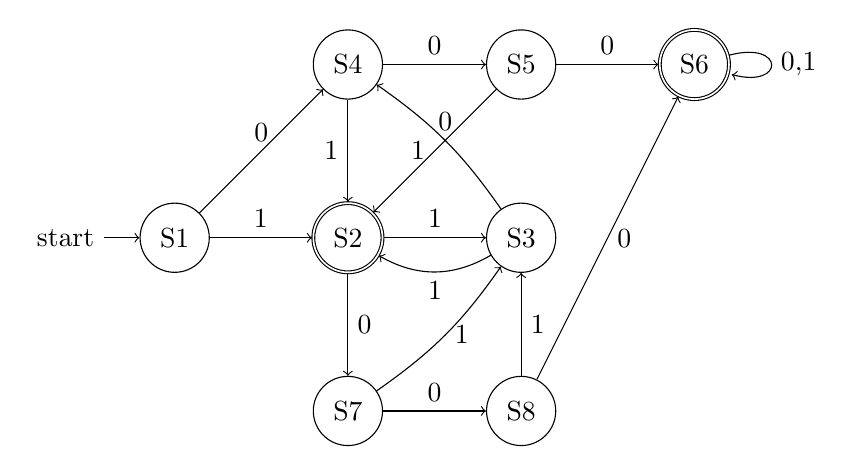
\begin{tikzpicture}[node distance=2.2cm, baseline]
				\node[state, initial] (s1) {S1};
				\node[state, accepting, right of=s1] (s2) {S2};
				\node[state, right of=s2] (s3) {S3};
				\node[state, above of=s2] (s4) {S4};
				\node[state, right of=s4] (s5) {S5};
				\node[state, accepting, right of=s5] (s6) {S6};
				\node[state, below of=s2] (s7) {S7};
				\node[state, right of=s7] (s8) {S8};
				\path[->] (s1) edge node [above] {1} (s2)
					(s1) edge node [above] {0} (s4)
					(s2) edge node [above] {1} (s3)
					(s2) edge node [right] {0} (s7)
					(s3) edge [bend left] node [below] {1} (s2)
					(s3) edge [bend right=10] node [above] {0} (s4)
					(s4) edge node [left] {1} (s2)
					(s4) edge node [above] {0} (s5)
					(s5) edge node [left] {1} (s2)
					(s5) edge node [above] {0} (s6)
					(s6) edge [loop right] node {0,1} (s6)
					(s7) edge [bend right=10] node [right] {1} (s3)
					(s7) edge node [above] {0} (s8)
					(s8) edge node [right] {1} (s3)
					(s8) edge node [right] {0} (s6);
			\end{tikzpicture}
			\item 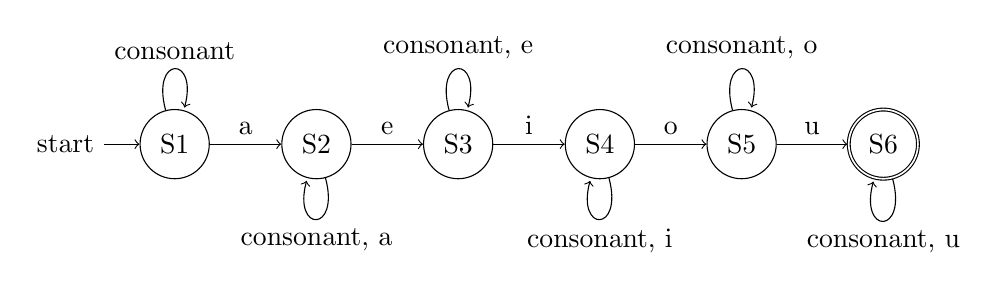
\begin{tikzpicture}[node distance=1.8cm,baseline]
				\node[state, initial] (s1) {S1};
				\node[state, right of=s1] (s2) {S2};
				\node[state, right of=s2] (s3) {S3};
				\node[state, right of=s3] (s4) {S4};
				\node[state, right of=s4] (s5) {S5};
				\node[state, accepting, right of=s5] (s6) {S6}; 
				\path[->] (s1) edge[loop above] node {consonant} (s1)
					(s1) edge node [above] {a} (s2)
					(s2) edge[loop below] node {consonant, a} (s2)
					(s2) edge node [above] {e} (s3)
					(s3) edge[loop above] node {consonant, e} (s3)
					(s3) edge node [above] {i} (s4)
					(s4) edge[loop below] node {consonant, i} (s4)
					(s4) edge node [above] {o} (s5)
					(s5) edge[loop above] node {consonant, o} (s5)
					(s5) edge node [above] {u} (s6)
					(s6) edge[loop below] node {consonant, u} (s6);
			\end{tikzpicture}
			\item 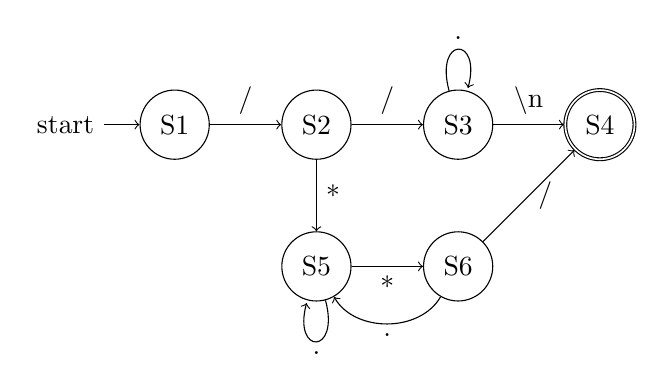
\begin{tikzpicture}[node distance=1.8cm, baseline]
				\node[state, initial] (s1) {S1};
				\node[state, right of=s1] (s2) {S2};
				\node[state, right of=s2] (s3) {S3};
				\node[state, accepting, right of=s3] (s4) {S4};
				\node[state, below of=s2] (s5) {S5};
				\node[state, right of=s5] (s6) {S6};
				\path[->] (s1) edge node [above] {/} (s2)
					(s2) edge node [above] {/} (s3)
					(s2) edge node [right] {*} (s5)
					(s3) edge [loop above] node {.} (s3)
					(s3) edge node [above] {\textbackslash n} (s4)
					(s5) edge [loop below] node {.} (s5)
					(s5) edge node [below] {*} (s6)
					(s6) edge [bend left=60] node [below] {.} (s5)
					(s6) edge node [right] {/} (s4);
			\end{tikzpicture}
		\end{enumerate}
		\item \begin{enumerate}
			\item 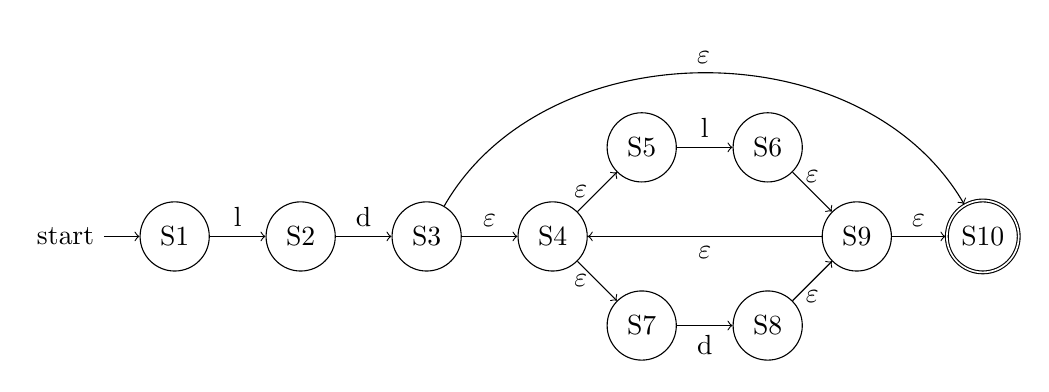
\begin{tikzpicture}[node distance=1.6cm, baseline]
				\node[state, initial] (s1) {S1};
				\node[state, right of=s1] (s2) {S2};
				\node[state, right of=s2] (s3) {S3};
				\node[state, right of=s3] (s4) {S4};
				\node[state, above right of=s4] (s5) {S5};
				\node[state, right of=s5] (s6) {S6};
				\node[state, below right of=s4] (s7) {S7};
				\node[state, right of=s7] (s8) {S8};
				\node[state, above right of=s8] (s9) {S9};
				\node[state, accepting, right of=s9] (s10) {S10};
				\path[->] (s1) edge node [above] {l} (s2)
					(s2) edge node [above] {d} (s3)
					(s3) edge node [above] {$\varepsilon$} (s4)
					(s3) edge [bend left=60] node [above] {$\varepsilon$} (s10)
					(s4) edge node [left] {$\varepsilon$} (s5)
					(s4) edge node [left] {$\varepsilon$} (s7)
					(s5) edge node [above] {l} (s6)
					(s6) edge node [above] {$\varepsilon$} (s9)
					(s7) edge node [below] {d} (s8)
					(s8) edge node [below] {$\varepsilon$} (s9)
					(s9) edge node [below] {$\varepsilon$} (s4)
					(s9) edge node [above] {$\varepsilon$} (s10); 
			\end{tikzpicture}
			\item 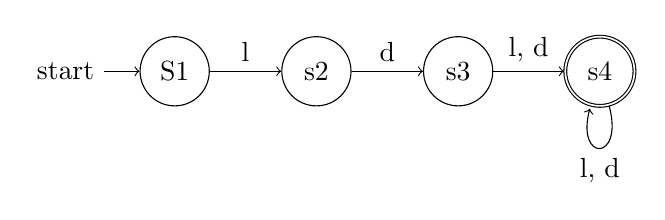
\begin{tikzpicture}[node distance=1.8cm, baseline]
				\node[state, initial] (s1) {S1};
				\node[state, right of=s1] (s2) {s2};
				\node[state, right of=s2] (s3) {s3};
				\node[state, accepting, right of=s3] (s4) {s4};
				\path[->] (s1) edge node [above] {l} (s2)
					(s2) edge node [above] {d} (s3)
					(s3) edge node [above] {l, d} (s4)
					(s4) edge [loop below] node {l, d} (s4);
			\end{tikzpicture}
		\end{enumerate}
	\end{enumerate}
\end{document}